\documentclass[12pt]{article}
\usepackage{graphicx}
\usepackage{color}
\usepackage{makeidx}
\usepackage{titlepic}
\usepackage{amssymb}
\usepackage{xspace}
\usepackage{amsmath}
\usepackage{bm}
\usepackage[numbers]{natbib}
%\usepackage[left=3cm,top=3cm,right=3cm,bottom=3cm]{geometry}
\usepackage{hyperref}

\title{On-line Option Discovery and De-Aliasing for Direct Policy Search}
\date{July 4, 2013}
\author{Laura Vogelaar}
\titlepic{\includegraphics{cover.png}}

\makeindex

\newcommand{\extract}[1]{{\em #1}}

\newcommand{\mymath}[1]{\ensuremath{#1}\xspace}

% Policy
\newcommand{\pol}    {\mymath{\pi}}
\newcommand{\act}    {\mymath{\mathbf{a}}}
\newcommand{\actsp}  {\mymath{\mathbf{A}}}
\newcommand{\sta}    {\mymath{\mathbf{s}}}
\newcommand{\stasp}  {\mymath{\mathbf{S}}}
% Parameterized policy
\newcommand{\app}    {\mymath{\bm{\theta}}}
\newcommand{\appsp}  {\mymath{\Theta}}
% Parameterized skill
\newcommand{\polg}   {\mymath{\Pi}}
\newcommand{\taskp}  {\mymath{\mathbf{q}}}
\newcommand{\taskpv} {\mymath{q}}
\newcommand{\taskpsp}{\mymath{Q}}
% Optimization
\newcommand{\costsp} {\mymath{R}}
\newcommand{\costf}  {\mymath{J}}
\newcommand{\covar}  {\mymath{\bm{\Sigma}}}
% Aliasing
\newcommand{\feat}   {\mymath{f}}
\newcommand{\featv}  {\mymath{\mathbf{f}}}
\newcommand{\featsp} {\mymath{\emph{F}}}
\newcommand{\obsm}   {\mymath{O}}

\DeclareMathOperator*{\argmin}{arg\,min}
\newcommand{\argminvar}[1]{\ensuremath{\underset{#1}{{\argmin}}}}

\begin{document}

\maketitle

\newpage
\thispagestyle{empty}
\mbox{}
\newpage
\vspace*{\fill}
{\color{red}
\textbf{\centerline{Notice of non-confidentiality:}}
{This document is not confidential. It can therefore be communicated externally in printed or electronic format.}
\newline
\newline
\textbf{\centerline{Note de non confidentialit\'{e}:}}
{Le document est non confidentiel. Il peut donc \^{e}tre communiqu\'{e} \`{a} l'ext\'{e}rieur sous format papier mais \'{e}galement diffus\'{e} sous format \'{e}lectronique.}
}
\vspace*{\fill}

\newpage
\vspace*{\fill}
\centerline{\textbf{Special Thanks}}
Special thank you to Freek Stulp for his mentorship and guidance throughout this internship experience.
\vspace*{\fill}
\newpage
\begin{abstract}
This is a report of a research internship performed at ENSTA ParisTech in the Robotics and Computer Vision Lab. The research goal was to design and determine the feasibility of a method for a robot to automatically distinguish when multiple tasks are being given and learn to perform them. The task used was for a simulated robot to lift various objects. At first the robot treated all perceived contexts as the same - known as perceptual aliasing. Then, based on given features of these objects and a measure of how successful the robot was after each action it tried, it created a mapping from perception to action, while at the same time optimizing all the actions. This method was successful when the actions for each task were similar and was not successful when the actions were very different. In conclusion, online de-aliasing uses a local search, but with a local method it is not possible to perform global de-aliasing.
\end{abstract}
\newpage
\tableofcontents
\newpage
\section{Introduction}

This internship was completed at \'{E}cole Nationale Sup\'{e}rieure de Techniques Avanc\'{e}es, Robotics and Computer Vision Lab under the supervision of Dr. Freek Stulp. The internship consisted of a research project, whose topic was how to autonomously de-alias perceptually-aliased tasks while running stochastic optimization. Dr. Stulp has been using stochastic optimization already in a variety of applications \cite{stulp12reinforcement}, and my goal was to add a way to create context-specific optimizers in instances where there are distinctly different contexts and actions. I worked directly under Dr. Stulp, and regular meetings between the two of us facilitated the development and direction of the project.

One of the longstanding difficulties in robotics is autonomously learning new skills to conquer different tasks. A human can distinguish that when presented with one particular situation, the best action may be different than when presented with another situation. Take the example of lifting a translucent milk carton. We've all experienced picking up an empty carton when we expected it to be full and suffering from overshooting and lifting the bottle too high. This shows that there are two different actions that are performed: one action for when the carton is empty, and one action for when the carton is full. It is only from our experience in lifting milk cartons that we know the fullness is the important feature on which to decide our action, not the color or the type of milk or any number of other irrelevant features. This mapping of relevant features to actions is called a ``perceptual class'' \cite{piater11learning}. Imagine now the case where the milk carton is opaque instead of translucent. There are still two actions that should be taken, one when the carton is full, and one when the carton is empty, but we can no longer distinguish the two perceptual classes since there are no relevant features. When two perceptual classes are being treated as one class, this is called perceptual aliasing. When perceptual aliasing is present, the best performance will either be an action that is a compromise in-between the two ideal actions that will work partially for both tasks, or one of the ideal actions that will work well for one task and poorly for the other task. 

The goal of this work is to start in a situation where we don't know that the fullness is what matters for picking up the milk carton, and we don't know that there are two tasks --- we start assuming there is only one task --- and to discover that there are two tasks, that they are defined by the fullness/emptiness, and what the ideal action is to take in both cases. This process is called perceptual de-aliasing since at first all perceptual classes are aliased, and the algorithm will split the perceptual class into non-aliased classes \cite{daniel12learning}. We will assume that there is at least one feature that can be used to detect each task (there is no opaque carton). The motivation is to perform perceptual de-aliasing online while also optimizing the action choices at the same time.

The experiments that were performed applied stochastic optimization and a perceptual de-aliasing technique first to a Dynamic Movement Primitive (DMP), and then to manipulation. For the DMP, the different tasks were different viapoints the trajectory must pass through. For manipulation, the different tasks were different objects that were to be lifted by a robot arm with a simple two finger gripper. The stochastic optimization algorithm and perceptual de-aliasing techniques will be discussed in further detail in the methods section.


\section{Formalization}
%policy

\subsection{Parameterized Policies and Policy Improvement}
\label{sec:parameterized_policies}

In reinforcement learning, a policy maps states to actions (\ref{eq:policy}). In continuous reinforcement learning, where the state space $\stasp \in \mathbb{R}^N$ and action space $\actsp \in \mathbb{R}^N$,  it is customary to use policies which are parameterized by a policy parameter vector \app in the space $\appsp  \in \mathbb{R}^N$.

\begin{align}
\label{eq:policy}     \pi:& \stasp               \mapsto \actsp & \mbox{Policy~} \pi(\act|\sta)\\
\label{eq:policy_par} \pi:& \stasp \times \appsp \mapsto \actsp & \mbox{Parameterized policy~} \pi(\act|\sta,\app)
\end{align}


Optimizing policy parameters with respect to a cost function is known as \emph{policy improvement}. 
One approach to policy improvement is to treat it as a black-box optimization problem. This means that no assumptions are made about the cost function $J$, and that $J$ returns only a scalar cost value. In this approach, the cost function maps the policy parameters to a scalar cost value~(\ref{eq:cost}). Policy parameters that minimize this cost function are known as optimal policy parameters $\app^*$~(\ref{eq:opt_pol_pars}).

\begin{align}
& \costf\mbox{: } \appsp \mapsto \mathbb{R}&\mbox{Cost function for policy improvement}\label{eq:cost}\\
& \app^* = \argminvar{\app}\costf(\app) \mbox{,~with~} \app\in\appsp  & \mbox{Optimal policy parameters}\label{eq:opt_pol_pars}
\end{align}

\subsection{Task Parameters}

The cost function definition in (\ref{eq:cost}) assumes that the cost is independent of the initial state, and that differences in cost are only caused by differences in \app. However, in robotics, the cost may well depend on the initial state, e.g. whether a robot successfully grasps an object depends not only the action of the robot, but also the position of the object. Therefore, we add the initial state to the cost function:

\begin{align}
& \costf\mbox{: } \appsp \times \stasp \mapsto \mathbb{R}&\mbox{Cost function with state}\label{eq:cost_state}
\end{align}

It is not necessarily the case that \emph{all} variables in the state space are relevant to the cost function. For instance, the color of an object does not usually matter for the success of the grasp. If all such irrelevant variables are removed from the state, we are left with the \emph{task parameters}. Formally, we define task parameter space \taskpsp as follows:
%
\begin{align}
s_i \in \taskpsp &\iff\notag\\
&\exists \sta \exists \sta' ~s_i\neq s'_i ~\wedge~\sta\backslash s_i= \sta'\backslash s_i ~\wedge~\notag\\
&\argminvar{\app}\costf(\app,\sta) \neq \argminvar{\app}\costf(\app,\sta')\label{eq:relq0} 
\end{align}

Thus, a state variable $s_i$ is a task parameter iff there are two state vectors whose components are all equal \emph{except} the component $s_i$, and these two state vectors require different policy parameters to minimize the cost function. Task parameters describe the initial state of the world before the policy is executed, and therefore do not change in time and do not include the robot's properties. If we exclude all irrelevant state variables from the state vector, we can thus rewrite our cost function as:

\begin{align}
\costf\mbox{: } &\label{eq:cost_task} \appsp \times \taskpsp \mapsto \mathbb{R}&\mbox{Cost function with task parameters}
\end{align}

\subsection{Including Task Parameters in Policies (Parameterized Skills)}

If (\ref{eq:relq0}) holds, then, to be optimal, different policy parameters are required for different task parameters. Optimal policies \emph{must} thus take the task parameters into account. 
Therefore, \emph{parameterized skills} calculate the policy parameters based on the task parameters in a seperate step:
%There are essentially two approaches to taking into account task parameters during the execution of the policy. The first is to pull the task parameters inside the parameterized policy:
%
%\begin{align}
%& \pol: \stasp\times\appsp\times\taskpsp \mapsto \actsp & \mbox{One-step parameterized skill $\pol(\act|\sta,\app,\taskp)$}
%\end{align}
%
%Examples of this approach include~\cite{matsubara11learning,  stulp13learning}. We will refer to these as `one-step' parameterized skills. The second approach is to intermediately compute the appropriate policy parameters for given task parameters with a \emph{policy parameter function}:

\begin{align}
\mbox{Step 1.~~}&\polg:\hat{\taskpsp}\mapsto\appsp & \mbox{Policy parameter function~} \polg(\app|\taskp)\label{eq:pol_par_fun}\\
\mbox{Step 2.~~}&\pol:\stasp\times\appsp\mapsto\actsp & \mbox{Action policy with parameters~}  \pol(\act|\sta,\app)
\end{align}

Now there is a two-level system: input task parameters into the policy parameter function which outputs policy parameters for the action policy, input these policy parameters to the action policy to perform the action. 

An important distinction is that Step 1. is performed off-line before the execution of the movement. It thus needs only take into account the values of the task parameter at the first time step $t=0$, and $\taskp \subset \sta_0$


\subsection{Policies with a Discrete set of Parameters (Options)}

One further distinction should be made with respect to the policy parameter function. In the first case, the policy parameter function maps to the continuous policy parameter space (\ref{eq:pol_par_fun_regr}). Example here zzz. For tasks of this nature, \polg is learned through regression~\cite{ude10taskspecific,matsubara11learning,silva12learning,stulp13learning}.
In the second case, when there are a discrete number of options for policy parameters (\ref{eq:pol_par_fun_class}), classification is used instead of regression for the policy parameter function.

\begin{align}
&\polg : \hat{\taskpsp} \mapsto \appsp & \mbox{Continuous} \label{eq:pol_par_fun_regr}\\
&\polg : \hat{\taskpsp} \mapsto \{\app_1,\app_2,\dots,\app_O\} \mbox{~with~} \app_i \in \appsp & \mbox{Discrete options} \label{eq:pol_par_fun_class}
\end{align}
% zzz 
% Continuous case: different optima for each task parameter
% Options case   : different optima at least one different task parameters, but not all.

\citet{daniel12learning} call this second type of policy parameter function an `option policy', because it is a policy for choosing from a set of options. A full list of the different terminologies for parameterized skills and the policy parameter function is provided in Section~\ref{sec:related_work}. 


\subsection{Perceptual Aliasing}

In this work, we are interested in automatically determining the number of options required, as well as the task parameters that are relevant to distinguishing between them. Unfortunately, the definition of task parameters in (\ref{eq:relq0}) does not enable the robot to determine the relevant task parameters in practice, because it requires an infinite number of evaluations of the cost function $J(\app,\sta)$. 
Thus, there is a distinction between the true task parameter space \taskpsp and the task parameter space as determined by the robot, which we denote $\hat{\taskpsp}$.
%Because it does not know the true task parameters of the cost function (\ref{eq:cost_task}), it also does not know which task parameters to include in the policy parameter function (\ref{eq:pol_par_fun}).
A problem arises when a state variable is relevant to the cost $s_i \in \taskpsp$, whereas the robot does not deem it to be relevant $s_i \in \hat{\taskpsp}$. In this case, the robot is not always able to determine the appropriate policy parameterizations for. This is known as \emph{aliasing}, which 
``[$\dots$] occurs when multiple situations that are indistinguishable [$\dots$] require different responses from the system.''~\cite{chrisman92reinforcement}.

Matters become even more complicated if one considers that the robot does not have direct access to the state either. Instead, we have access to the detectable features.  The feature space contains the set of all possible feature vectors that can be seen. Each feature within this vector can be either a real number or one of a discrete set. In the robot example, the features might be the color of the object, in which case its value is one of a discrete set such as \{red, yellow, blue\}, or it could be the color intensity measured by a sensor, in which case it would be a continuous numeric value. The features which are observed are a function of the state \eqref{eq:obs}. The color sensor value would be a function of the object's color, and the visual data would be a function of the object's geometry and orientation with respect to the camera, and so on.

\begin{align}
\obsm\mbox{: } &\label{eq:obs}\stasp \mapsto \featsp& \mbox{Observation model~} \featv=\obsm(\taskp)\\
\featsp &= \featsp_1 \times \featsp_2 \times ... \times \featsp_N & \mbox{Feature space}\\
\mbox{with~} &\featsp_i \in \mathbb{R}\mbox{, or~} \featsp_i \in \{C_1,C_2,...,C_N\}&\notag%\\
%\featv &\in \featsp\mbox{, with~} \featv = <\feat_1,\feat_2,...,\feat_n>&
\end{align}


Thus, the policy parameter function and parameterized policy must be rewritten as follows: 

\begin{align}
\mbox{Step 1.~~}&\polg:\featsp\mapsto\appsp & \mbox{Policy parameter function~} \polg(\app|\featv)\label{eq:pol_par_fun}\\
\mbox{Step 2.~~}&\pol:\featsp\times\appsp\mapsto\actsp & \mbox{Execute policy with parameters~}  \pol(\act|\featv,\app)
\end{align}

Not being able to distinguish, based on features alone, which situations require different actions is known as \emph{perceptual aliasing}, where ``Perceptual aliasing occurs when multiple situations that are indistinguishable from immediate perceptual input require different responses from the system.''~\cite{chrisman92reinforcement}.
We formalize this concept as follows.
First of all, relevant features in the space $\featsp_Q$ can only generated by task parameters, which are the task-relevant part of the state.
\begin{align}
\obsm_Q\mbox{: } &\label{eq:obs_task}\taskpsp \mapsto \featsp_Q \mbox{~with~} \featsp_Q \subset \featsp \mbox{~and~}  \taskpsp \subset \stasp
\end{align}

% zzz Something about not caring about F\F_q, and finding enough features in F_Q to make the relevant distinctions.

%It is necessary to define the idea of relevance: what makes a feature or a task parameter relevant? A task parameter is relevant when it can take on different values that will lead to different optimal actions \eqref{eq:relq}. We are assuming that there is a task parameter that independently influences the cost. It is possible that a case could arise where only changing two cost parameters at once causes a different action to be taken, but we are not considering that at this time. 

%\begin{align}
%\taskp_i =& <\taskpv_1,\taskpv_2,...,\taskpv_i,...\taskpv_N> \notag & 
%\\
%\taskp'_i =& <\taskpv_1,\taskpv_2,...,\taskpv'_i,...\taskpv_N> \notag & \taskpv_i \neq \taskpv'_i \\
%\label{eq:relq} \taskp_i \in \taskpsp_{REL} \iff&\argminvar{\app}\costf(\app,\taskp_i) \neq \argminvar{\app}\costf(\app,\taskp'_i)\\
%\taskpsp_{REL} \cup & \taskpsp_{IRR} = \taskpsp,   \taskpsp_{REL} \cap \taskpsp_{IRR} = \emptyset 
%\end{align}
%
%Multiple tasks are present when \eqref{eq:relq} is true since there are two ideal actions. Therefore there are multiple tasks present if and only if there is at least one relevant task parameter. If a difference in one or more of the features can be detected when the task parameter changes, then it will be possible to perceptually de-alias the two tasks. Since the goal is to de-alias in an online fashion, the ideal action, $\argminvar{\app}\costf(\app,\taskp)$, will not be known at the moment of de-aliasing. Instead, the value of the cost function $\costf$ is used as an indicator by how different it is for different values of the task parameter in question \eqref{eq:relq} as to whether or not the ideal action will be different in the two cases. Sometimes this will lead to overzealous de-aliasing, but perceptual classes can easily be merged again if it is discovered the same actions are being performed.

\section{Methods}

\subsection{Evolution Strategies for Policy Improvement}
\label{sec:evolution_strategies}

As defined in Section~\ref{sec:parameterized_policies}, the goal of policy improvement is to find the optimal policy parameters $\app^*$ which minimize the cost function $J:\appsp \mapsto \mathbb{R}$.

Stochastic optimization relies on exploring the input space of the cost function, which in the case of policy improvement is the policy parameter space. To foster exploration, we define a stochastic policy as follows:

\begin{align}
& \pi(\act|\sta,\app_\mu,\covar) & \mbox{Stochastic policy} \label{eq:stoch}
\end{align}

where the mean $\app_\mu$ and covariance matrix \covar  define a normal distribution. When executing the policy, a specific policy parameter vector \app is sampled from a normal distribution with the mean $\app_\mu$ and the variance $\covar$ shown, and executed with \app. This is known as parameter space exploration. 

Stochastic optimization proceeds by taking $K$ policy parameter samples~(\ref{equ_so_sample}), and determining the cost for each of these samples by executing the policy~(\ref{equ_so_cost}). Then, costs are converted into weights $w_k$, where samples with lower costs have higher weights. In~(\ref{equ_so_wa_mean}) the new mean of the distribution is computed through a weighted averaging over the samples. Low-cost samples thus contribute more to the new mean then high-cost samples, and the the mean $\app_\mu$ thus (on average) moves closer to $\app^*$. The same is done for the covariance matrix.

\begin{align}
\app_{k=1\dots K} & {\sim}\mathcal{N}({\app_\mu},{\covar})\label{equ_so_sample}\\
\forall k~J_k & = J(\app_k) \label{equ_so_cost}\\
\forall k~w_k & = \mbox{``lower cost} \Rightarrow \mbox{higher weight''}\label{equ_so_cost_to_w}\\
\app_\mu^{new} & = \sum_{k=1}^{K} w_k \app_k\label{equ_so_wa_mean}\\
\covar^{new} & = \sum_{k=1}^{K}w_k(\app_k-\app_\mu)(\app_k-\app_\mu)^\intercal\label{equ_so_wa_covar}
\end{align}

This procedure iterates until a halting criteria. For deterministic environements, the resulting optimal policy is also deterministic, i.e. \covar=$\mathbf{0}$:

\begin{align}
& \pi(\act|\sta,\app^*,\mathbf{0}) & \mbox{Optimal (deterministic) policy} \label{eq:stoch_opt}
\end{align}

\subsection{Perceptual De-aliasing}
The following description will be given in the context of the simulated robot which will be discussed further later in the paper, but this algorithm can be equally well applied to performing and action which is defined by a discrete number of parameters. 

The robot is given an initial starting motion through imitation learning. Then the robot will choose K sample actions, in which each action parameter is taken from a normal distribution centered around the imitation learning value and with a predefined initial covariance matrix. When the robot is next required to perform a task, it will record the features present, perform a sample action from the distribution, and record the cost that it incurs. Now after each performed task, the robot will accumulate a roll-out which contains the perception, action parameters, and cost. After K tasks have been seen, the sampling distribution and sampling covariance matrix are updated, biased towards the lower cost actions. Now future action will be drawn from this new sampling distribution. 

If there is only one task, the algorithm will proceed in this manner, performing stochastic optimization until the local minimum of the cost is found, presumably towards perfecting the demonstrated action. If there are two tasks being shown, which have similar but different actions that need to be performed then this algorithm by itself will never find the context-specific best actions. Therefore, task splitting needs to be introduced in order to detect the difference between two different tasks. After this distinction is made, the two tasks can be treated separately, each with its own sampling distribution. To implement this idea, after K samples are taken, but before the new distribution is updated, a splitting test is run to determine if there are two different tasks that are falsely being treated as the same task.

\begin{figure}[ht]
  \centering
  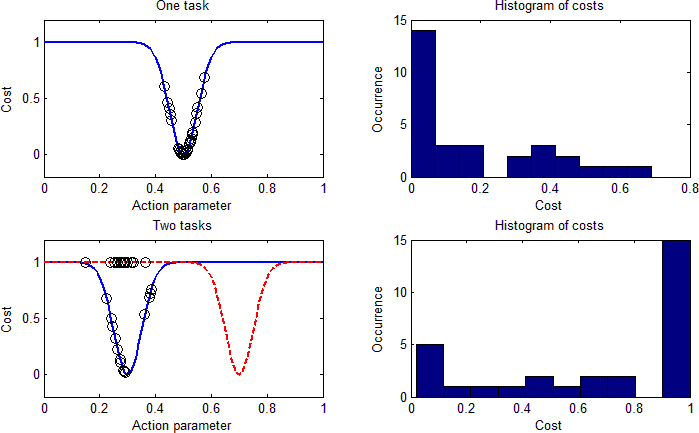
\includegraphics[width=0.9\columnwidth]{one_vs_two_tasks.png}
  \caption{One versus two tasks}
  \label{fig:1vs2tasks}
\end{figure} 

In Figure \ref{fig:1vs2tasks}, the top two plots show the situation where there is only one task, i.e. $\taskpsp_1 = \taskpsp$. The bottom two plots shows the situation where there are two tasks. The blue line shows $\costf(\app,\taskp), \taskp \in \taskpsp_1$

\color{red}Each task has its own cost function. When two tasks are being treated as the same task, some of the samples will be the cost function from one task, and some will be the cost function from the other task. \color{black} When the sampling distribution is at a location where the two cost functions vary, a histogram of the costs will reveal that there are two different clusters. By looking only at the cost distribution, regardless of the action taken, we are assuming that the action taken does not matter. In the case where the covariance matrix for the sampling distribution is small, this serves as a fairly accurate estimation, since all the actions taken in the K samples are very similar. Once the costs are clustered, any supervised learning algorithm can be used to determine which features indicate which cluster. For this work, a classification tree was used. If we had followed in a similar thread as~\citet{piater11learning}, the parallel would have been to determine visual classes by using the covariance matrix. If the covariance matrix remained large, or moved back and forth repeatedly, we could assume this was due to visual class aliasing, but it may also happen by chance, and is dependent on the reinforcement learning algorithm. Instead, by using approximately equivalent actions as if they were the same action, visual classes can be found completely independently of the reinforcement algorithm used. 

Once a new visual class is identified by the supervised learning algorithm, the sampling distribution and covariance is initialized as the sampling distribution of both tasks before the split. If the cost function for both tasks is smooth and has a non-zero gradient at all points, the new optimizer should be able to find the minimum for the new task. 




%\subsection{Task Splitting Techniques}

Once a sufficient number of similar actions were taken, the percept-action-cost data was collected. Since the action was very similar, it could be taken as constant, reducing the complexity to percept-cost. Treating each perceived feature individually yielded a two dimensional work space of feature value vs. cost. 

\subsubsection{Gaussian Mixture Models in Cost-Feature Space}

The two dimensions of feature and cost were plotted against each other and then fitted with a Gaussian Mixture Model [4]. This was done in an attempt to see if there were two Gaussians, and whether they were very different in cost-space and percept-space. Upon further reflection, this only works with truly continuous features, and not with binary or classification features, since in this case, the `value' given in the feature space is meaningless as far as its spacial relation to its neighbors.

\begin{figure}[ht]
  \centerline{
  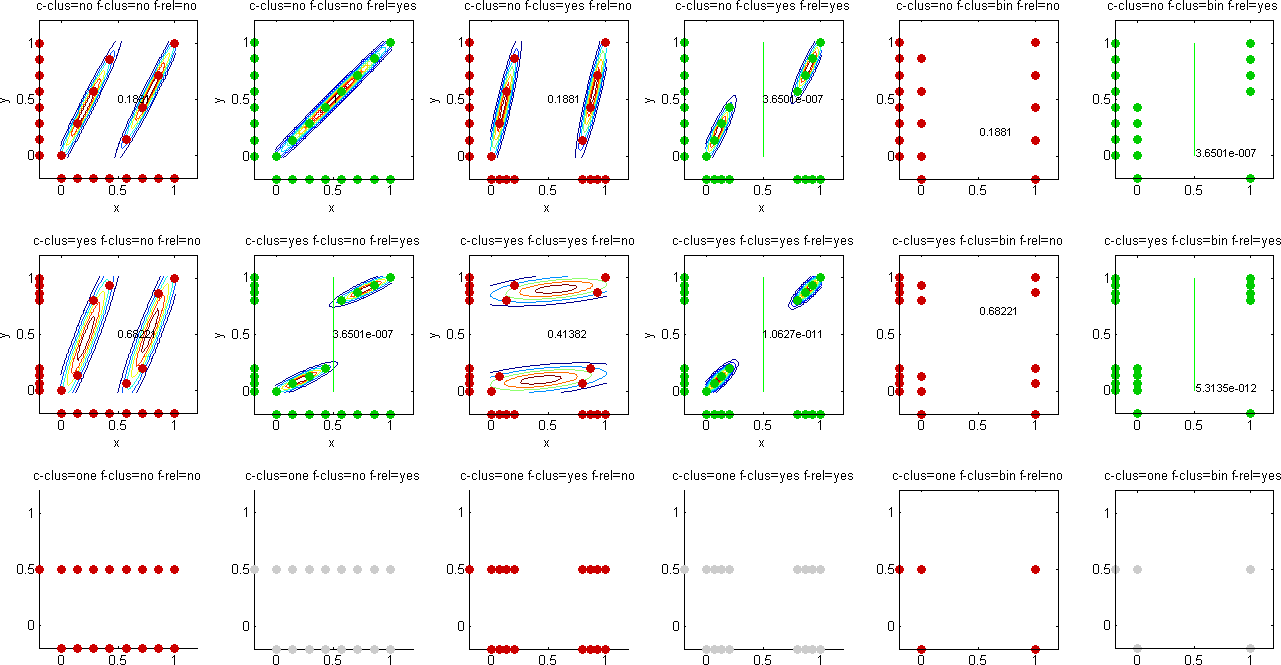
\includegraphics[width=1.0\columnwidth]{2d_gaussians.png}}
  \caption{\label{fig_2d_gaussians} 2D Gaussian Mixture Model performance on idealized data}
  \label{fig:2Dgaussians}
\end{figure}


\subsubsection{Clustering Costs}

In this technique, the one-dimensional cost vector is clustered in order to see if there are two separate cost functions being seen. If the clusters are significantly different from one another (determined by a Student T-test), then a classification tree is used to find the feature combination that leads to the cluster membership function. Since relevant features are assumed in this experiment, the classification tree is pruned to one layer and then tested to see if it still correctly predicts the membership function to within a defined threshold. If it does, then the feature used is relevant and defines two visual classes with different cost functions. If it does not, then the clustering of the costs indicates that there may be two different cost functions, but that with the given features, it is impossible to distinguish the two tasks. 

The technique of fitting 2D Gaussian distributions is only applicable to situations where the feature is continuous. In Figure \ref{fig:2Dgaussians}, several idealized situations were subjected to this splitting method. The green plots show situations in which a split should ideally be detected, and the red are cases were a split should not be detected. The headings c-clus and f-clus, refer to whether the costs are clusterable and whether the feature itself is clusterable, respectively. When there is a green vertical line on the plot, this indicates that the algorithm decided to split this data, and the location of this line on the x-axis is the cutoff point for the feature that was chosen. For the binary features, 2D Gaussian fitting is not necessary since the variance in the feature space will be zero, thus these situations are decided using a paired Student T-Test with different variances. Figure \ref{fig:clustercosts} shows the results of the clustering algorithm performed on the same set of idealized data. This time the cost must be clusterable in order to find a split, but it will work on categorical data and is more robust. 


\begin{figure}[ht]
  \centerline{
  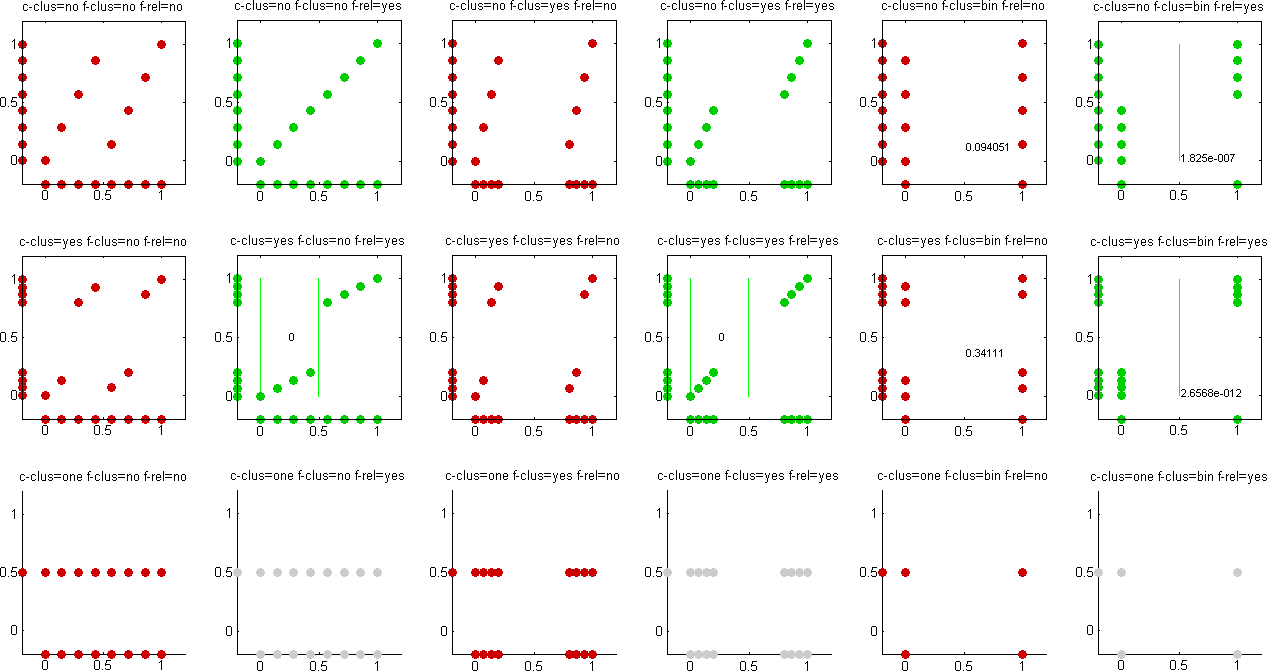
\includegraphics[width=1.0\columnwidth]{cluster_costs.png}}
  \caption{\label{fig_cluster_costs} Cost Clustering performance on idealized data}
  \label{fig:clustercosts}
\end{figure}

\subsubsection{Covariance Divergence}


\section{Results}

\subsection{Viapoint Task}

\subsection{Robot Arm Simulations}
\subsubsection{Experiment Setup}

\begin{figure}[ht]
  \centering
  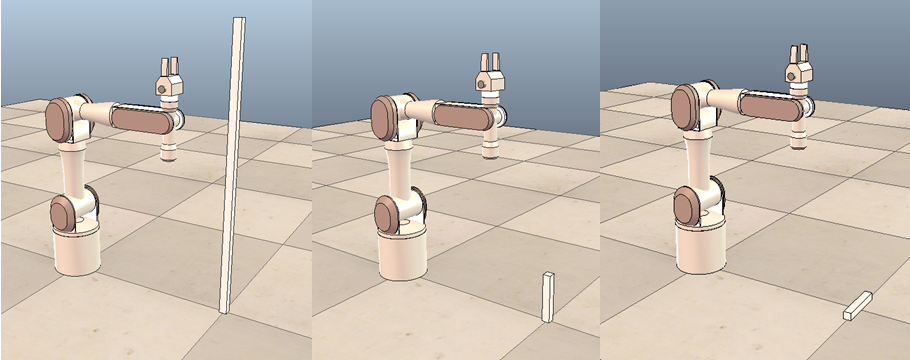
\includegraphics[width=0.9\columnwidth]{robots.png}
  \caption{\label{fig_robots} Left: tall standing rod. Center: short standing rod. Right: short laying-down rod.
  \label{fig:robots}
  }
\end{figure}

The robot simulator V-REP was used to simulate a robot arm with a simple two finger, one degree of freedom gripper. The action space was six-dimensional, and controlled the end position and orientation of the gripper. After the desired end position was reached, the gripper closed, and the arm lifted a predefined amount. The task was to lift an object that was placed before the robot always at the same coordinates. The cost of a trial was given by the weighted combination of how high the object was lifted, how little the orientation of the object changed throughout the lifting, and the minimum distance between the gripper and the surface of the object through the entire motion. The last part of this cost function was added to help compensate for the large number of actions that would have had a constant high cost due to the robot not coming into contact with the object at all. Adding this component allowed for the robot to naturally move closer to the object, until the orientation or lifting success, which were weighted higher, made the part of the cost due to distance negligible. 

	The following pairs of tasks were given to the robot to be solved:
	
Setup 1:	Tall standing rod	vs.	Short standing rod

Setup 2:	Short standing rod	vs. 	Short laying-down rod

	Initially both tasks were treated as if they were one visual class. The initial action distribution was given manually as a successful grasp for one of the two tasks. Once aliasing was detected, the two visual classes were defined by one of the perception variables and optimized independently.
	
Successful grips between the tall standing rod and the short standing rod are very similar. The action parameter is different in only one dimension, and not very far within this dimension. Therefore this situation is more like that discussed on the left half of Figure \ref{fig:costfunction}, where there is cost information for both tasks that overlaps. For this reason, the two skills were successfully found and optimized. In the case of the laying-down rod, the action parameters were similar in three dimensions, but very different in three other dimensions. A different pose was needed to grasp the rod from above instead of from the side since it was lying down. This situation corresponds to the right half of Figure \ref{fig:costfunction}, where the cost information for the two tasks is distinct and far away, making it impossible to use the local aliased solution to find the very different global solution.

\subsubsection{Experiment Results}

\begin{figure}[ht]
  \centerline{
  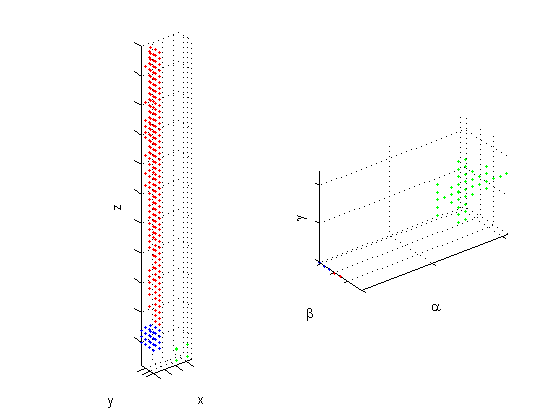
\includegraphics[width=0.9\columnwidth]{6d.png}}
  \caption{\label{fig_6d} Successful policy parameters divided by task. Red is tall standing rod, blue is short standing rod, and green is short laying-down rod.}
  \label{fig:6d}
\end{figure}

Setup 1 resulted in a split based on the height of the rod. The final action for the tall standing rod was to lift from the center of mass, and the final action for the short standing rod was the lift from just below the top of the rod. Both moves were successful and yielded low costs. Setup 2 also resulted in a split. The final action for the short standing rod was the same as in Setup 1, but the final action for the laying-down rod was an unsuccessful grip similar to that of the short standing rod. What happened in Setup 2 was that the two tasks were correctly identified by a percept variable and split accordingly, but the two tasks required such different actions to be successful that the gap could not be overcome. To further demonstrate this idea, refer to Figure \ref{fig:6d}, which shows the successful trials of each of the three tasks being performed. The tall standing rod is shown in red, the short standing rod in blue, and the short laying-down rod in green. Since this task is 6-dimensional, it is not easy to show all dimensions at once. Instead, on the left are the \emph{x},\emph{y}, and \emph{z} linear dimensions, and on the right are the angular dimensions, \emph{$\alpha$},\emph{$\beta$}, and \emph{$\gamma$}. 

\begin{figure}[ht]
  \centering
  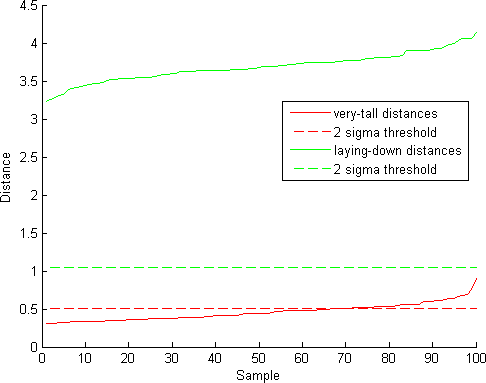
\includegraphics[width=0.8\columnwidth]{distance.png}
  \caption{\label{fig_distance} Comparison of distances between the short standing rod task and the other two tasks in action space.}
  \label{fig:distance}
\end{figure}

\newpage
While the three tasks seem quite close to one another in linear space, it is clear that the laying-down rod is very distant from the other two tasks in angular space. This distance explains why the correct action was found between the two standing rods, but not between a standing and a laying-down rod. Since the short standing rod was used as the initial imitation-learned solution, we can measure the likelihood that a sample taken from here will reach a successful grasp for one of the other tasks. One hundred samples were taken with a reasonable covariance matrix and the initial mean of the short standing rod. The Euclidean distance between these samples and the two other tasks was then calculated. In Figure \ref{fig:distance} these distances are plotted, with the 2 sigma cutoff around each task's optimal action. The very tall rod successfully has many samples within range of its optimal action. The laying-down rod does not have any samples anywhere close to being within range. The optimal actions are too different from each other that one solution will not provide any information about the other solution.

\subsection{Global Optima with Local Search}

However, in real applications, even if the cost function is smooth, there is often only a small range of action parameters near the solution which give any useful feedback. Still using a Gaussian cost function, but this time with a cut-off of two sigma, and in 2D, the cost function could be one of the following two cases. Either there is a large overlap between the non-constant regions of the two cost functions, or there is no overlap between the non-constant regions. In the case of overlap, it is feasible that once splitting occurs, some of the samples of the second distribution will land in a non-constant cost region, thus leading the skill towards the solution. In the case where there is no overlap, the probability of a sample getting a non-constant cost is very small. Without some variability in the costs, the skill will move in a random direction and due to the covariance update methods, will eventually stop, and miss the solution.
 
\begin{figure}[ht]
  \centering
  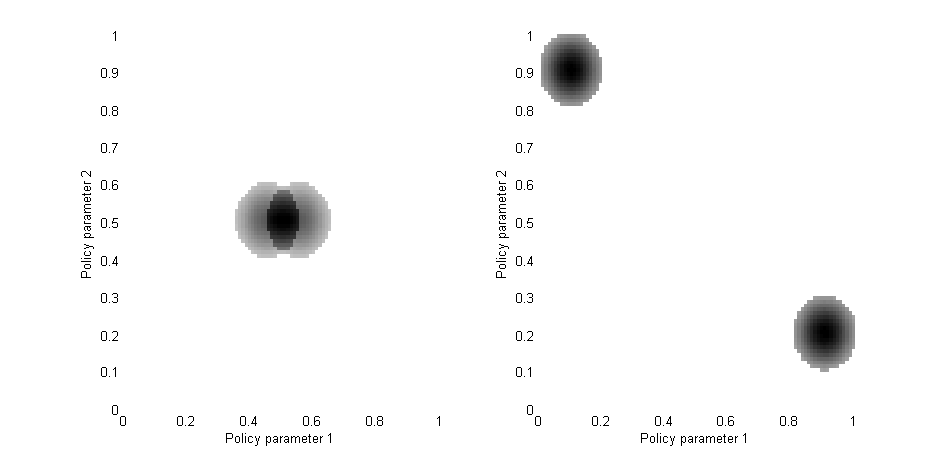
\includegraphics[width=0.9\columnwidth]{cost_function.png}
  \caption{ Possible cost functions for two tasks. Left: likely to find both optimal actions due to overlap. Right: unlikely to find both optimal actions due to large distance between the two optimal actions.}
  \label{fig:costfunction}
\end{figure}

\begin{figure}[ht]
  \centering
  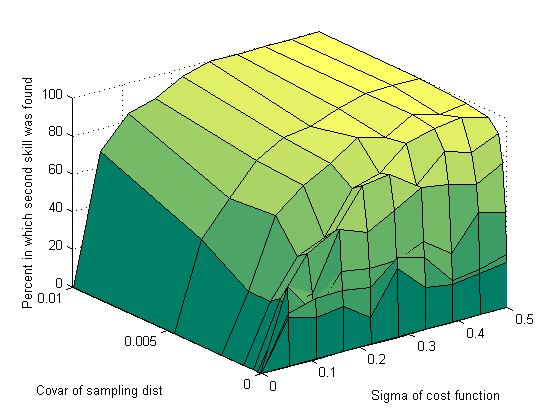
\includegraphics[width=0.6\columnwidth]{sigma_vs_covar.png}
  \caption{\label{fig_sigma_vs_covar} Success rate of finding two ideal actions, when the cost function is non-constant within a range of 2 Sigma, and the samples are taken from a sampling distribution with the the shown covariance. }
  \label{fig:sigmavscovar}
\end{figure}

Figure \ref{fig:costfunction} shows two examples of this experiment, one in which we would expect both minima to be found (left), and the other (right) which it is unlikely the second minima will be found. The dark circles indicate low-cost areas, and the white background is a constant high-cost area. Splitting will only occur when there is a difference in the cost values of the two tasks for the current action. This means splitting cannot occur in the white portion of the graphs, it can only occur in non-equivalent regions. Therefore, once split, there will be a large gap between the current action and the ideal action for one of the tasks. Figure \ref{fig:sigmavscovar} shows the percentage that both minima are successfully found when varying the sampling covariance and the cost distribution's standard deviation. The likelihood of finding the second skill diminishes when the cost distribution's standard deviation is reduced because the probability of drawing a sample within the 2-sigma radius funnel is lower. In a real life problem, the dimensionality will be very high, the funnel mouth very small, and the search space very large. It is logical to conclude that unless the two skills are very close in all dimensions of the action space, that the probability of finding the second skill is negligible. This conclusion is supported by the results of my experiment.

\section{Related Work}
\label{sec:related_work}

\subsection{Reinforcement Learning of Parameterized Policies}

\citet{stulp12reinforcement}

\subsection{Reinforcement Learning of Parameterized Skills}

\citet{stulp13learning}
\citet{kupcsik13dataefficient}
\citet{marin12towards}
\citet{matsubara11learning}

\subsection{Reinforcement Learning of Option Policies}

\citet{daniel12learning}

\subsection{Perceptual De-Aliasing in Reinforcement Learning}

\citet{chrisman92reinforcement}
\citet{mccallum95instancebased}
\citet{piater11learning}


\citet{marin12towards}


\color{red}
\subsection*{Humanoids'13}

\citet{ude10taskspecific} learn parameterized skills with a combination of Locally Weighted Regression (for the shape parameters) and Gaussian Process Regression (for the other skill parameters). 
\citet{silva12learning} use a combination of ISOMAP and Support Vector Machines. 
An interesting aspect of \cite{silva12learning} is that different regressors are learned for different parts of the parameter space, thus avoiding the problem of averaging across multiple skill parameters that achieve the same task. For instance, reaching around an obstacle will succeed  by going around it to the left \emph{or} right, but the average of these two motions will not succeed. 

\citet{matsubara11learning} also move the task parameters (which they call `style parameter') into the function approximator of a DMP. An interesting aspect of~\cite{matsubara11learning} is that task parameters are not provided, but rather extracted from the data itself through principal components analysis.

\citet{kober10reinforcement} present an altogether different approach for learning to map task parameters to DMP meta-parameters based on cost-regularized kernel regression. They consider the shape parameters to be fixed, and learn only the meta-parameters.

\color{black}

\color{red} Explain Gennaro's work here \color{black}


\begin{table}[ht]
  \centering
\begin{scriptsize}
\begin{tabular}{|l|l|rl|rl|rl|}
%-------------------------------------------------------------------------
%-------------------------------------------------------------------------
\hline
\multicolumn{8}{|l|}{\em Parameterized skills: Two-step methods}\\
%-------------------------------------------------------------------------
This report                          
& $\pol(\act|\sta,\app)$ 
& {\bf task pars}            & \taskp 
& {\bf policy pars}          & \app 
& {\bf policy pars function} & $\polg: \taskpsp \mapsto \appsp$ ($\polg: \taskp \mapsto \app$)\\  
%-------------------------------------------------------------------------
\citet{ude10taskspecific}      
& not specified
& task pars            & $\mathbf{q}$ 
& policy pars          & $[\mathbf{w},\tau,g]$ 
& function             & $\mathbf{G}: \mathbf{q} \mapsto [\mathbf{w},\tau,g]$ \\  
%-------------------------------------------------------------------------
\citet{kupcsik13dataefficient} 
& $\pi(\mathbf{u}|\mathbf{x},\mathbf{\omega})$ 
& context              & $\mathbf{s}$
& policy pars          & $\mathbf{\omega}$ 
& upper level policy   & $\pi(\mathbf{\omega}|\mathbf{s})$ \\  
%-------------------------------------------------------------------------
\citet{silva12learning}        
& $\pi_\mathbf{\theta}$
& task pars            & $\mathbf{\tau}$ 
& policy pars          & ${\theta}$
& parameterized skill  & $\Theta: T \mapsto \mathbb{R}^N$ ($\Theta: \mathbf{\tau} \mapsto \mathbf{\theta}$)\\
%-------------------------------------------------------------------------
%-------------------------------------------------------------------------
\hline
\multicolumn{8}{|l|}{\em Parameterized skills: One-step methods}\\
%-------------------------------------------------------------------------
\citet{matsubara11learning}    
& $f(x,\mathbf{s}; \mathbf{W})$
& style pars           & $\mathbf{s}$ 
& \multicolumn{2}{c|}{N.A.}   
& \multicolumn{2}{c|}{N.A.} \\  
%-------------------------------------------------------------------------
\citet{stulp13learning}        
& $h_\mathbf{u}(s,\mathbf{q})$
& task pars            & $\mathbf{q}$ 
& \multicolumn{2}{c|}{N.A.}   
& \multicolumn{2}{c|}{N.A.} \\  
%-------------------------------------------------------------------------
%-------------------------------------------------------------------------
\hline
\multicolumn{8}{|l|}{\em Option policies}\\
%-------------------------------------------------------------------------
\citet{daniel12learning}    
& $\pi(\mathbf{a}|\mathbf{s},o)$
& \multicolumn{2}{c|}{N.A. ($\approx\mathbf{s}$)}   
& option           & $o$ 
& gating network   & $\pi(o|\mathbf{s})$ \\  
%-------------------------------------------------------------------------
%-------------------------------------------------------------------------
\end{tabular}
\end{scriptsize}
  \caption{\label{tab_nomenclature} Different nomenclature in related work on parameterized skills with trajectory-based policy representations.}
\end{table}




\citet{daniel12learning} described an approach at IROS 2012  that used relative entropy policy search with hierarchical policy representations. They are not exactly using perceptual classes, but are finding multiple solutions to a single task. For their algorithm, a number of options are predefined, greater than the number of possible optima, and redundant options are deleted as the algorithm runs, with care taken to avoid premature deletion. Their robot playing tetherball example uses a 29-dimensional action space $\appsp$, and imitation learning is used to set the initial parameters of the dynamic motion primitive (DMP). It is not clear if these options all have the same initial policy, or if they are seeded differently. By starting with a large number of redundant options, it is more likely that they will cover the action space and find the possible solutions than if using a single option and then splitting into new options. While this may be feasible for a small number of basis functions, when it is a larger search space, the number of needed initial perceptual classes will increase rapidly. 

\citet{calinon13compliant} uses a Gaussian Mixture Model to estimate the structure of the cost function \costf, mapping the cost as a function of action as if it were a probability density function. In their experiment, only one task was shown, so accordingly there were no task parameters, and the cost function was reduced to $\costf(\app)$ instead of the full $\costf(\app,\taskp)$. Their experiment uses an action space that is 2-dimensional. In very large and high-dimensional action spaces, it will require a very large number of samples to accurately estimate the cost function's Gaussian Mixture Model. To tackle the problem of finding global optimums with a local search, \citet{calinon13compliant} employ decaying exploration noise. If the exploration noise is too low or zero, the optimizer would become trapped in the local minima, and not explore the rest of the cost function.

Task-specific representations were explored by~\cite{piater11learning} in which perception-action solutions were created by interleaving a percept classifier with a reinforcement learner. Effectively this means that while the reinforcement learner is trying to optimize the task at hand, the percept classifier is trying to parse out the perceptual classes. Once the perceptual classes are distinguished, the reinforcement learner will work independently on each of the newly defined perceptual classes. The reinforcement method they used was Markov Decision Processes (MDP). Their method for de-aliasing was to determine if the ideal action $\app$ was converging or not. They measured this convergence by seeing if the difference errors between subsequent iterations of the MDP updates were getting smaller or not. This method is the logical parallel to the Mean Divergence technique I tested. They assume any failure to converge directly is caused by aliasing, and not due to possible inherent instability in the system. They concede that their experiments were run in very small action-spaces $\appsp$, and that scalability may not be feasible. 


\section{Conclusion}

Online de-aliasing will work when the actions that need to be taken in different contexts are near to each other in action-space. This supports the fact that if the robot is trying to learn two movements that are very different, learning one of them does not give any information on how to do the other. Clustering the costs after a number of similar actions successfully allows the determination of visual classes and provides the advantage of not requiring a bond between the chosen reinforcement algorithm (in this case stochastic optimization) and the chosen supervised learning algorithm (in this case decision trees). In the situations where online de-aliasing works, the actions are very similar and based on the perceptual context. This occurs usually when the action is parameterized by the relevant perceptual feature. Future work would be to combine discretized visual classes that can be formed by online de-aliasing into perceptually parameterized skills.

%\bibliographystyle{plain}
\bibliographystyle{plainnat}
\bibliography{final_report}


\end{document}
